%%%%%%%%%%%%%%%%%%%%%%%%%%%%%%%%%%%%%%%%%%%%%%
\section{Run Plan}
\label{sec:runplan}

To formulate a preliminary run plan, we assume the hadron beam spectrum and rates are as given in Tables~\ref{tab:beampartcomp} and~\ref{tab:beampartrates}.   For the purpose of estimating the beam time request, an average trigger/data rate of 50 Hz to tape is assumed.
\fixme{IMPORTANT: you should assume 25 Hz for any data run duration estimates and requests!  Otherwise we may find ourselves in a situation where we can only record ~50\% of our envisaged samples; on the other hand if we manage to run at 50Hz we'll always find other useful things to do ...}

 
For the run scenario where we take 10K beam spills (two 4.8 sec spills per SPS Super-cycle) for each momentum bin from 1 to 7 GeV/c at 1 GeV/c step, the resulting sample for the positive beam is shown in Table~\ref{tab:RunPlan}. 

\begin{cdrtable}[Run Plan]{cccccccc}{RunPlan}{A preliminary run plan for ProtoDUNE-SP. The expected sample (positive beam) as a function of momentum is shown. }
P (GeV/c) & \# of spills &\# of $e^+$ & \# of $K^+$ & \# of $\mu^+$ & \# of $p$ & \# of $\pi^+$ & Total \# of Events \\ \toprowrule
1 & 10K & 672K & $\approx$ 0 & $\approx$ 0 & 192K & 144K & 1M \\ \colhline
2 & 10K & 480K & $\approx$ 0 & $\approx$ 0 & 336K & 480K & 1.3M \\ \colhline
3 & 10K & 1.5M & 17K  & 17K                & 203K  & 642K  & 2.4M \\ \colhline
4 & 10K & 1.1M & 49K & 33K                 & 197K & 1M & 2.4M \\ \colhline
5 & 10K & 896K  & 64K  & 16K               & 208K  & 1.2M & 2.4M \\ \colhline
6 & 10K & 667K & 99K  & 14K                & 241K  & 1.4M & 2.4M \\ \colhline
7 & 10K & 502K & 110K & 24K                & 257K  & 1.5M & 2.4M \\ \colhline
 & & & & & & & \\
Total & 70K & 5.9M & 340K & 104K & 1.6M & 6.4M & 14M \\
\end{cdrtable}

Similar table is also expected for the negative beam sample. 

Preliminary beam simulations show that the hadron rates at 
energies below 1~GeV/c are low. Moreover, low energy beams are more
subject to disruption and degradation by materials in the
beamline. Therefore, the beam program factors in the beam composition and also takes
into account of particle interaction topologies.  Full FLUKA\cite{fluka05,Fluka15}
 simulations
of particle transport in the the ProtoDUNE detector, including the
beam window, have been performed.
 The physics requirement is the possibility to measure
 stopping particles and  interactions both at high and at low energies.    
%For stopping, the “initial “energy has small meaning
At 1 GeV/c, still 35\% of protons do stop, while they reduce to only 5
per mill at 2 GeV/c.  At  1 GeV/c  the protons interact at all
energies as shown in
Figure~\ref{fig:pandpiint}. The residual energy at the interaction
point can be reconstructed by measuring the energy deposit along the proton track.
Many of the  low energy pions decay in the 37~m between the secondary target
and the LAr volume.  The fraction of stopping $\pi$ for one $\pi$
leaving the target is 3\% at P=0.4~GeV/c still  1.3\% at P=0.7~GeV/c,
then decreases.  Having a $\pi$ beam at 0.7~GeV/c still allows to
measure pion interactions down to few tens of MeV with good
statistics. In a 1~GeV/c beam, the low energy interactions are still
present albeit with lower rate, as shown in Figure~\ref{fig:pandpiint}.
%\fixme{also need to address particle interaction topologies}
As for Kaons, the length of the beam line is such that no
$K$ arrives at the detector for momenta lower than $\approx$2~GeV/c.
As for electrons, the peculiar topology of very low energy electron initiated 
showers requires a measurement at the lowest possible momenta.
\begin{cdrfigure}[Energy at interaction]{pandpiint}{Kinetic energy of
    particles at the point of interaction in the ProtoDUNE active
    volume, for different beam momenta. Histograms are normalized to one particle injected in the
    beamline acceptance. FLUKA simulations include the beam window
    materials, beam are considered as monochromatic and
    parallel. left: protons, right: pions.}
  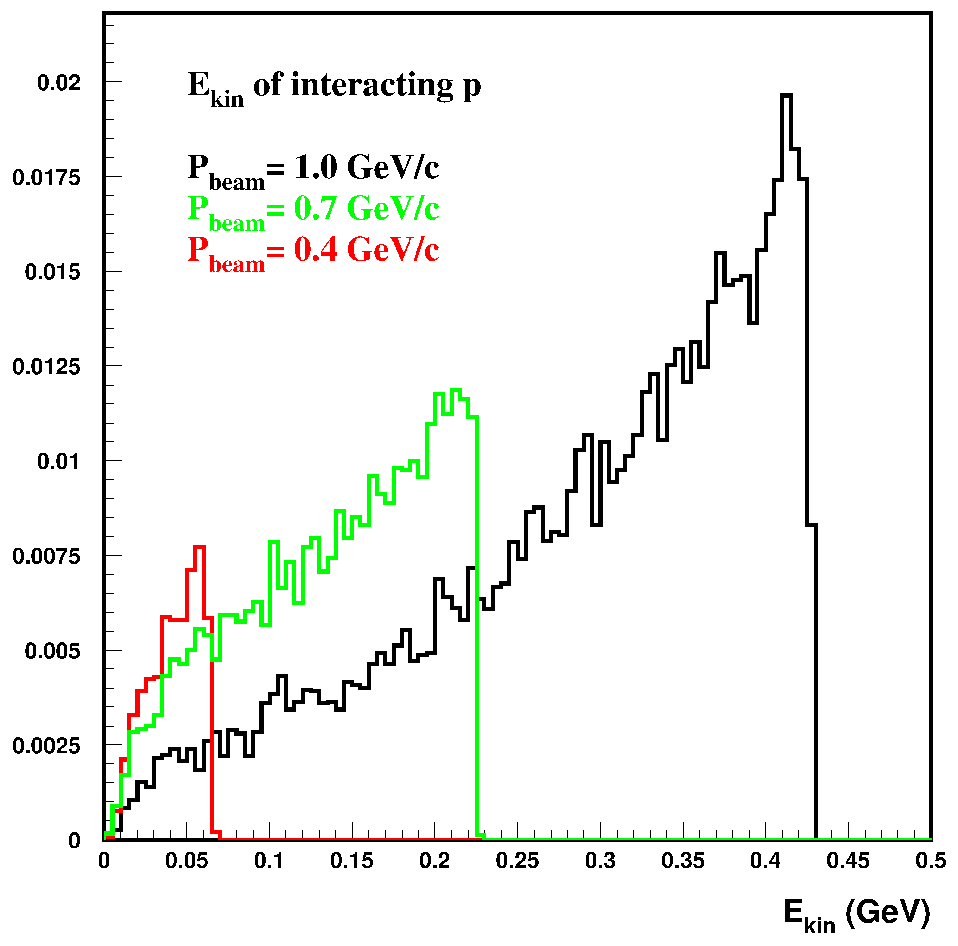
\includegraphics[width=0.49\textwidth]{pvarie_intene.pdf}
  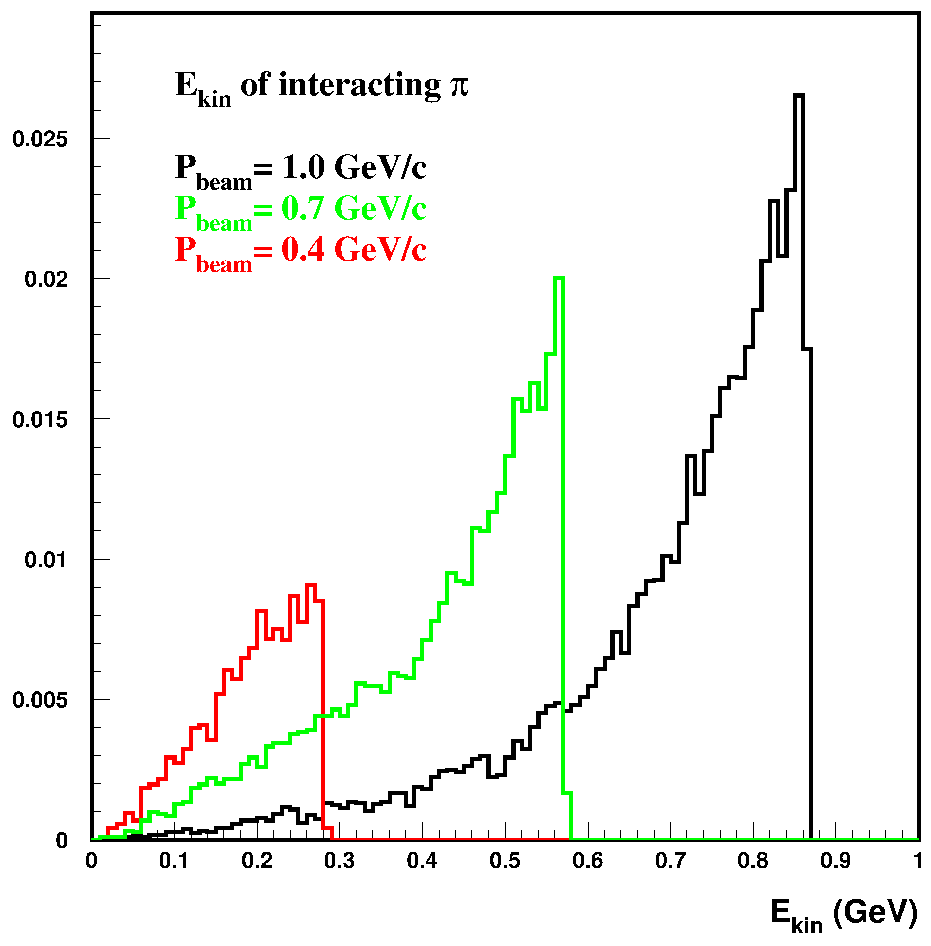
\includegraphics[width=0.49\textwidth]{pivarie_intene.pdf}
\end{cdrfigure}
%% end of   part that can go either here or in the run plan 

\fixme{Please make a separate table with estimates for $<$1 GeV hadrons and also electrons.}

In addition to the hadron beam run, there is an option to take some electron samples down to 0.5 GeV/c if requested by the physics group. 
\fixme{This has already been requested - please include it in your run plan.}
Based on the current information available, the total estimated beam time needed to carry out the physics program in this proposal is on the order of 6 weeks.
\fixme{never underestimate the beam time you need; err on the high side !}
 
 



